\hypertarget{peeragogy}{%
\subsection{Peeragogy}\label{peeragogy}}

\hypertarget{motivation}{%
\subsection{Motivation}\label{motivation}}

This pattern is relevant to anyone who wants to do active learning
together with others in a relatively non-hierarchical setting.

\hypertarget{context}{%
\subsection{Context}\label{context}}

Collaborative projects like Wikipedia, StackExchange, and FLOSS
represent an implicit challenge to the old ``industrial'' organization
of work. This new way of working appears to promise something more
resilient, more exciting, and more humane. The rhetoric has been
questioned {{[}3,9{]}}. In and across these ``free'', ``open'',
post-modern organizations, individual participants are learning
{{[}7{]}} -- and that they collectively change the methods and
infrastructure as they go. Because everyone in these projects primarily
learns by putting in effort on a shared work-in-progress, participants
are more in touch with an \emph{equality of intelligence} than an
\emph{inequality of knowledge} {{[}4:38, 119{]}}. At the same time, they
invoke a form of friendly competition, in which \emph{the best
craftmanship wins} {{[}5:89{]}}.

\hypertarget{forces}{%
\subsection{Forces}\label{forces}}

\begin{quote}
\Sthreshold\ \textbf{Threshold}: inclusiveness
and specificity are in tension.\\
\Strust\ \textbf{Trust}: is only built through
sharing and reciprocity.
\end{quote}

\hypertarget{problem}{%
\subsection{Problem}\label{problem}}

Even a highly successful project like Wikipedia is a work in progress
that can be improved to \emph{better} empower and engage people around
the world, to develop \emph{richer and more useful} educational content,
and to disseminate it \emph{more} effectively -- and deploy it more
creatively.\footnote{\url{https://wikimediafoundation.org/wiki/Mission_statement}}
How to go about this is a difficult question, and we don't know the
answers in advance. There are rigorous challenges facing smaller
projects as well, and fewer resources to draw on. Many successful free
software projects are not particularly collaborative -- and the largest
projects are edited only by a small minority of users {{[}2,10{]}}. Can
we work smarter together?

\hypertarget{solution}{%
\subsection{Solution}\label{solution}}

The act of asking ``can we work smarter together?'' puts learning front
and center. Peeragogy takes that ``center'' and distributes it across a
pool of heterogeneous relationships. Indeed, peeragogy can be understood
as an up-to-date revision of Alexander's {{Network of Learning}}
{{[}1:99{]}}. It \emph{decentralizes the process of learning and
enriches it through contact with many places and people} in
interconnected networks that may reach all over the world. Importantly,
while people involved in a peeragogical process may be collaborating on
{{A specific project}}, they don't have to be direct collaborators
outside of the learning context or co-located in time or space. Just as
theories and practices of pedagogy articulate the transmission of
knowledge from teachers to students, peeragogy articulates the way peers
produce and use knowledge together (Figure {[}fig:connections{]}).

\hypertarget{rationale}{%
\subsection{Rationale}\label{rationale}}

The peeragogical approach particularly addresses the problems of small
projects stuck in their individual silos, and large projects becoming
overwhelmed by their own complexity. It does this by going the opposite
route: explicating \emph{what by definition is tacit} and employing
\emph{a continuous design process} {{[}8:9--10{]}}. As Howard Rheingold
remarks in the foreword to the \emph{Peeragogy Handbook}: ``What made
this work? Polycentric leadership is one key'' {{[}6:iii{]}}.
``Peer-led'' shouldn't suggest that there are no leaders: rather, it
means that multiple leaders act as peers.

\hypertarget{resolution}{%
\subsection{Resolution}\label{resolution}}

Peeragogy helps people in different projects describe and solve real
problems. If you share the problems that you're experiencing with
others, there's a reasonable chance that someone may be able to help you
solve them. Bringing a problem across the \textbf{threshold} of someone
else's awareness helps achieve clarity. This process can guide
individual action in ways that we wouldn't have seen on our own, and may
lead to new forms of collective action we would never have imagined
possible. People who gain experience comprehending problems together
build \textbf{trust}. Making room for multiple right answers contributes
further to resolving the tension between generality and specificity.

\hypertarget{example-1}{%
\subsection{Example 1}\label{example-1}}

Wikipedia and its sister sites Wiktionary, Wikiversity, etc.
(collectively ``Wikimedia'') rely on user-generated content, peer
produced software, and are managed, by and large, by a pool of users who
choose to get involved with governance and other ``meta''
duties.\footnote{\url{https://www.wikimedia.org/}} The Wikimedia
Foundation maintains the servers and acts on behalf of this ``global
movement''. They achieve something quite impressive: Wikipedia is the
7th most popular website in the world, but the Wikimedia Foundation has
under 300 employees. For comparison, the 6th (Amazon) and 8th (QQ) most
popular websites are run by companies with over 200K and 28K employees,
respectively.\footnote{\url{https://en.wikipedia.org/wiki/Wikimedia_Foundation\#Employees}},\footnote{\url{http://phx.corporate-ir.net/phoenix.zhtml?c=97664\&p=irol-newsArticle\&ID=2100418}},\footnote{\url{https://www.google.com/finance?cid=695431}},\footnote{\url{http://www.alexa.com/topsites}}

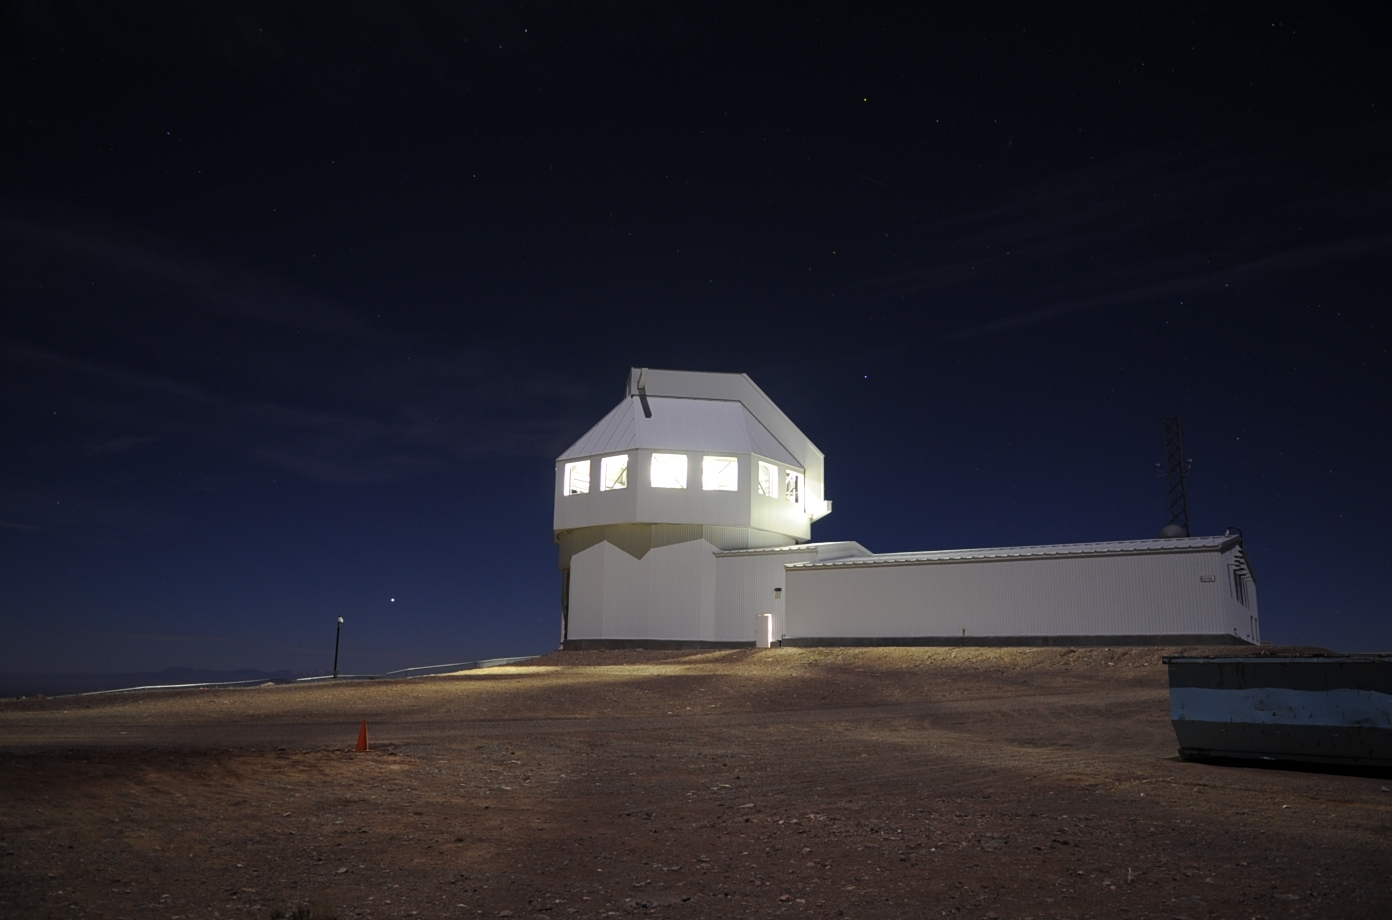
\includegraphics{images/Space_Surveillance_Telescope.jpg}
\emph{Observatory : Space Surveillance Telescope, New Mexico.}

\hypertarget{example-2}{%
\subsection{Example 2}\label{example-2}}

Although one of the strengths of {{Peeragogy}} is to distribute the
workload, this does not mean that infrastructure is irrelevant. The
students and researchers of the future university will need access to an
Observatory and other scientific apparatus if they are to reach \emph{ad
astra, per aspera} (Figure 1).\footnote{Latin: ``With difficulty, to the
  stars.''}

\hypertarget{whats-next-in-the-peeragogy-project}{%
\subsection{What's Next in the Peeragogy
Project*}\label{whats-next-in-the-peeragogy-project}}

We intend to revise and extend the \emph{Patterns of Peeragogy} into a
framework that can describe and scaffold the learning that happens
inside and outside of institutions.

\hypertarget{references}{%
\subsection{References}\label{references}}

\begin{enumerate}
\def\labelenumi{\arabic{enumi}.}
\item
  Christopher Alexander, Sara Ishikawa, and Murray Silverstein. 1977.
  \emph{A Pattern Language: Towns, Buildings, Construction}. Oxford
  University Press, Oxford.
\item
  Benjamin Mako Hill. 2011. When Free Software Isn't (Practically)
  Better. Retrieved from
  \url{http://www.gnu.org/philosophy/when_free_software_isnt_practically_better.html}
\item
  Daniel Kreiss, Megan Finn, and Fred Turner. 2011. The limits of peer
  production: Some reminders from Max Weber for the network society.
  \emph{New Media \& Society} 13, 2: 243--259.
\item
  Jacques Rancière. {[}1987{]} 1991. \emph{The ignorant schoolmaster:
  Five lessons in intellectual emancipation}. Stanford University Press.
\item
  Eric S Raymond. 2001. \emph{The Cathedral \& the Bazaar: Musings on
  Linux and open source by an accidental revolutionary}. O'Reilly Media,
  Inc.
\item
  H. Rheingold and others. 2015. \emph{The Peeragogy Handbook}.
  PubDomEd/Pierce Press, Chicago, IL./Somerville, MA. Retrieved from
  \url{http://peeragogy.org}
\item
  J. P. Schmidt. 2009. Commons-Based Peer Production and education.
  \emph{Free Culture Research Workshop, Harvard University}: 1--3.
  Retrieved from
  \url{http://cyber.law.harvard.edu/fcrw/sites/fcrw/images/Schmidt_Education_FreeCulture_25Oct2009.pdf}
\item
  Till Schümmer, Joerg M Haake, and Wolfgang Stark. 2014. Beyond
  rational design patterns. \emph{Proceedings of the 19th european
  conference on pattern languages of programs}, ACM, 13 pp.
\item
  Aaron Shaw and Benjamin Mako Hill. 2014. Laboratories of Oligarchy?:
  How the iron law extends to peer production. \emph{Journal of
  Communication} 64, 2: 215--238.
\item
  Aaron Swartz. 2006. Who Writes Wikipedia? Retrieved from
  \url{http://www.aaronsw.com/weblog/whowriteswikipedia}
\end{enumerate}

\begin{center}\rule{0.5\linewidth}{0.5pt}\end{center}

\hypertarget{notes}{%
\subsection{Notes}\label{notes}}
